%%% Econ712: Macroeconomics I
%%% Fall 2020
%%% Danny Edgel
%%%
% Due on Canvas Thursday September 24, 11:59pm Central Time
%%%

%%%
%							PREAMBLE
%%%

\documentclass{article}

%%% declare packages
\usepackage{amsmath}
\usepackage{amssymb}
\usepackage{array}
\usepackage{bm}
\usepackage{changepage}
\usepackage{centernot}
\usepackage{graphicx}
\usepackage{fancyhdr}
	\fancyhf{} % sets both header and footer to nothing
	\renewcommand{\headrulewidth}{0pt}
    \rfoot{Edgel, \thepage}
    \pagestyle{fancy}
	
%%% define shortcuts for set notation
\newcommand{\N}{\mathbb{N}}
\newcommand{\Z}{\mathbb{Z}}
\newcommand{\R}{\mathbb{R}}
\newcommand{\Q}{\mathbb{Q}}
\newcommand{\lmt}{\underset{x\rightarrow\infty}{\text{lim }}}
\newcommand{\neglmt}{\underset{x\rightarrow-\infty}{\text{lim }}}
\newcommand{\zerolmt}{\underset{x\rightarrow 0}{\text{lim }}}
\newcommand{\loge}[1]{\text{ln}\left(#1\right)}
\newcommand{\usmax}[1]{\underset{\{#1\}}{\text{max }}}

%%% define column vector command (from Michael Nattinger)
\newcount\colveccount
\newcommand*\colvec[1]{
        \global\colveccount#1
        \begin{pmatrix}
        \colvecnext
}
\def\colvecnext#1{
        #1
        \global\advance\colveccount-1
        \ifnum\colveccount>0
                \\
                \expandafter\colvecnext
        \else
                \end{pmatrix}
        \fi
}

%%% define function for drawing matrix augmentation lines
\newcommand\aug{\fboxsep=-\fboxrule\!\!\!\fbox{\strut}\!\!\!}

\makeatletter
\let\amsmath@bigm\bigm

\renewcommand{\bigm}[1]{%
  \ifcsname fenced@\string#1\endcsname
    \expandafter\@firstoftwo
  \else
    \expandafter\@secondoftwo
  \fi
  {\expandafter\amsmath@bigm\csname fenced@\string#1\endcsname}%
  {\amsmath@bigm#1}%
}


%________________________________________________________________%

\begin{document}

\title{	Problem Set \#3 }
\author{ 	Danny Edgel 					\\ 
			Econ 712: Macroeconomics I		\\
			Fall 2020						\\
		}
\maketitle\thispagestyle{empty}

%%%________________________________________________________________%%%

\noindent\textit{Collaborated with Sarah Bass, Emily Case, Michael Nattinger, and Alex Von Hafften}


%%%________________________________________________________________%%%

\section*{Question 1}
We are given:
\begin{align*}
	U(c_t,c_{t+1}^t)&=\loge{c_t^t}+\loge{c_{t+1}^t}	\\
	U(c_1^0) &= \loge{c_1^0}
\end{align*}
Where each generation is endowed with $w_1$ when young and $w_2<w_1$ when old, and the initial old generation is endowed with $\overline{M}>0$ units of fiat currency. Each generation has a unit measure of agents.

\begin{itemize}
	\item[(a)] In each period, the social planner faces the problem:
		\[
			\usmax{c_t^t,c_t^{t-1}}\loge{c_t^t} + \loge{c_t^{t-1}} \text{ s.t. } c_t^t + c_t^{t-1} \leq w_1 + w_2
		\]
		Note that this includes the initial old geneation's allocation in time $t=1$. Since the objective function is increasing in both $c_t^t$ and $c_t^{t-1}$, the budget constraint is an equality. Solving for $c_t^{t-1} = w_1 + w_2-c_t^t$, we can solve:
		\begin{align*}
			&\usmax{c_t^t}\loge{c_t^t} + \loge{w_1 + w_2-c_t^t} \\
			\text{ F.O.C. } &\frac{1}{c_t^t} - \frac{1}{w_1+w_2-c_t^t} = 0	\\
							&c_t^t = w_1 + w_2 -c_t^t 						\\
							&c_t^t = \frac{1}{2}(w_1 + w_2)
		\end{align*}
		Therefore, the social planner's problem is solved by the allocation:
		\[
			\{c_1^0,\{c_t^t,c_t^{t=1}\}_{t=1}^\infty\}=\left\{\frac{1}{2}(w_1 + w_2),\left\{\frac{1}{2}(w_1 + w_2),\frac{1}{2}(w_1 + w_2)\right\}_{t=1}^\infty\right\}
		\]
		
	\item[(b)] In this model, there are two representative households: the initial old generation, and each generation $t=\{1,2,...\}$. Then, the household problem is:
		\begin{align*}
			\usmax{c_1^0}\loge{c_1^0}												\text{ s.t. } 	&c_1^0		\leq w_2 + \frac{\overline{M}}{p_1}	\\
			\usmax{\{c_t^t,c_{t+1}^t,M^t_{t=1}\}}\loge{c_t^t} + \loge{c_{t+1}^t}	\text{ s.t. } 	&c_t^t 		\leq w_1 - \frac{M_{t+1}^t}{p_t}	\\
																									&c_{t+1}^t 	\leq w_2 + \frac{M_{t+1}^t}{p_{t+1}}
		\end{align*}
		
	\item[(c)] An autarkik equilibrium for this model is a set of prices, $\{p_1,\{p_t,p_{t+1}\}_{t=1}^\infty\}$, and an allocation, $\{c_1^0,\{c_t^t,c_t^{t=1}\}_{t=1}^\infty\}$ such that in every period, each agent consumes their own endowment and all markets clear:
		\begin{align*}
			&M_t = \overline{M}				&\text{(Money Market)} \\
			&c_t^t + c^{t-1}_t = w_1 + w_2 	&\text{(Goods Market)} 
		\end{align*}
		There is no savings technology and agents do not trade in autarky, so to solve for the equilibrium allocation, we simply set each agent's consumption equal to their endowment in each period:
		\[
			\{c_1^0,\{c_t^t,c_t^{t=1}\}_{t=1}^\infty\}=\left\{w_2,\left\{w_1,w_2\right\}_{t=1}^\infty\right\}
		\]
		Now, we can use our allocation and the market-clearing conditions to solve for the market-clearing prices and the money allocation. Since each agent's objective function is increasing in consumption, they meet their budget constraint in each period. Then, setting consumption equal to endowment for each agent in each period:
		\begin{align*}
			w_2 &= w_2 + \frac{\overline{M}}{p_1}	\\
			w_1 &= w_1 - \frac{M_{t+1}^t}{p_t}		\\
			w_2 &= w_2 + \frac{M_{t+1}^t}{p_{t+1}}
		\end{align*}
		Therefore, $\frac{\overline{M}}{p_1}=\frac{M_{t+1}^t}{p_t}=\frac{M_{t+1}^t}{p_{t+1}}=0$. The equilibrium set of prices in autarky is $\left\{\frac{1}{p_t}\right\}=0$.
		
	\item[(d)] Let $w_2=0$ and assume that money is valued. Then, the competitive equilibrium is, again, an allocation and set of prices such that the goods and money market clear. We can derive these values by solving each representative agent's household problem. Since the initial old generation consumes only in period $t=1$ and their utility is increasing on $c_1^0$, we can derive that $c_1^0=w_2 + \frac{\overline{M}}{p_1}$. Using the budget contraint of the generation $t\geq 1$ problem, we can solve:
		\begin{align*}
			\usmax{M_{t+1}^t}	&\loge{w_1-\frac{M_{t+1}^t}{p_t}} + \loge{\frac{M_{t+1}^t}{p_{t+1}}}									\\
			\text{F.O.C.: }		&-\frac{1}{p_t\left(w_1-\frac{M_{t+1}^t}{p_t}\right)} + \frac{1}{p_{t+1}\frac{M_{t+1}^t}{p_{t+1}}} = 0	\\
								&p_{t+1}w_2 + M^t_{t+1} = p_t m_1 - M_{t+1}^t															\\
								&M_{t+1}^t = \frac{1}{2}(p_tw_1-p_{t+1}w_2) = \frac{1}{2}p_tw_1
		\end{align*}
		Using our definition of $M_{t+1}^t$ with respect to consumption in each period, we can derive:
		\begin{align*}
			c_t^t 		&= w_1-\frac{1}{2p_t}(p_tw_1-p_{t+1}w_2) = \frac{1}{2}\left(w_1 + \frac{p_{t+1}}{p_t}w_2\right) = \frac{1}{2}w_1					\\
			c_{t+1}^t 	&= w_2 + \frac{1}{2p_{t+1}}(p_tw_1 - p_{t+1}w_2) = \frac{1}{2}\left(\frac{p_t}{p_{t+1}}w_1 + w_2\right) = \frac{p_t}{2p_{t+1}}w_1
		\end{align*}
		Thus, our goods market clearing condition enables us to solve:
		\begin{align*}
			c_t^t + c^{t-1}_t = \frac{1}{2}w_1 + \frac{p_{t-1}}{2p_t}w_1 	&= w_1	\\
								1 + \frac{p_{t-1}}{p_t}						&= 2	\\
								\frac{p_{t-1}}{p_t}							&= 1	\\
								p_{t-1}										&= p_t
		\end{align*}
		While the money market clearing condition combines with $c_1^0=w_2 + \frac{\overline{M}}{p_1}$ and the equation for $M_{t+1}^t$ to determine the initial old generation's consumption in $t$:
		\begin{align*}
			M_2^1 				&= \overline{M}	\\
			\frac{1}{2}p_1w_1 	&= p_1c_1^0		\\
			c_1^0				&= \frac{1}{2}w_1
		\end{align*}
		Which is consistent with our finding for $c^{t-1}_t$ for an arbitrary $t\geq 1$ Thus, the allocation of the competitive equilibrium in this model is:
		\[
			\{c_1^0,\{c_t^t,c_t^{t=1}\}_{t=1}^\infty\}=\left\{\frac{1}{2}w_1,\left\{\frac{1}{2}w_1,\frac{1}{2}w_1\right\}_{t=1}^\infty\right\}
		\]
		
	\item[(e)] The table below displays the equilibrium allocations of initial old generation and the representative agents from generation $t$ and $t-1$ at time $t$ in each of the three scenarios (social planner's problem, autarky, monetary), each assuming that $w_2 = 0$. The social planner's allocation is achieved in the monetary economy, but in autarky, all old generations experience zero consumption, leading to an aggregate negative infinity utility level in every period.
		\begin{center}
			\begin{tabular}{r|c c c}
							& $c_0^1$			& $c_t^t$ 			& $c_t^{t-1}$			\\
				\hline		&					&					&						\\
				SPP			& $\frac{1}{2}w_1$	& $\frac{1}{2}w_1$	& $\frac{1}{2}w_1$		\\
				Autarky 	& 0					& $w_1$				& 0						\\
				Monetary	& $\frac{1}{2}w_1$	& $\frac{1}{2}w_1$	& $\frac{1}{2}w_1$
			\end{tabular}
		\end{center}
		
	\item[(f)] If the initial money supply were halved, the direct impact would occur in the budget constraint of the initial old generation, which would become:
		\[
			c_1^0 \leq \frac{\overline{M}}{2p_1}
		\]
		Since the initial old generation's utility is increasing in consumption, this budget constraint will hold with equality in equilibrium. For agents in generation $t\geq 1$, the optimal choice of $M_{t+1}^t$ does not depend directly on the initial money supply. Thus, when money markets clear, we can solve:
		\begin{align*}
			M_2^1 				&= \frac{\overline{M}}{2}	\\
			\frac{1}{2}p_1w_1 	&= p_1c^0_1					\\
			\frac{1}{2}w_1 		&= c^0_1
		\end{align*}
		Neither the optimal choice of $\{c_t^t,c_{t+1}^t\}$ nor the goods market clearing condition depend on the initial money supply, so, as in the previous monetary solution, $\{c_t^t,c_{t+1}^t\}=\{\frac{1}{2}w_1,\frac{1}{2}w_1\}$. Thus, the equilibrium allocation does not change when the initial money supply is halved.
		
\end{itemize}


%%%________________________________________________________________%%%

\section*{Question 2}
The trade offer curves for each utility function given, using the given endowments, are plotted below.

\begin{itemize}
	\item[(a)] $U=10c_1-4c_1^2 + 4c_2-c_2^2$, $(w_1,w_2)=(0,2)$
		\smallskip \\
		As the chart below shows, the indifference curves for the utility function are ellipses.
		\begin{center}
			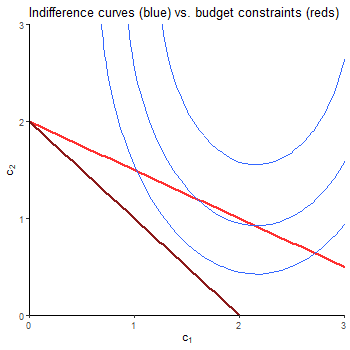
\includegraphics[scale=.6]{2a_IC-and-BC.png}
		\end{center}
		Maximizing utility under each budget contraint (determined by the ratio of prices between each good) results in an asymmetric quasi-parabola which, because $w_1=0$, is bounded by $x_1\geq 0$ but never reaches a boundary point where $c_2=w_2$:
		\begin{center}
			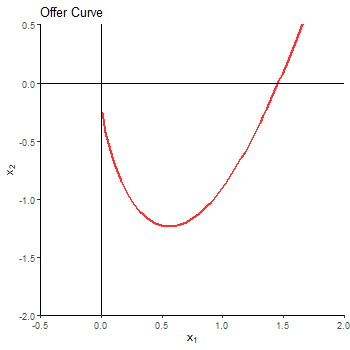
\includegraphics[scale=.6]{2a_offer-curve.png}
		\end{center}
		
	\pagebreak
	\item[(b)] $U=\text{min}\{2c_1+c_2,c_1+2c_2\}$, $(w_1,w_2)=(1,0)$
		\smallskip \\
		The indifference curves for this utility function are shaped like tilted, obtuse angles, reflecting the complementary nature of $c_1$ and $c_2$. The graph below displays the indifference curves and budget constraints of this problem.
		\begin{center}
			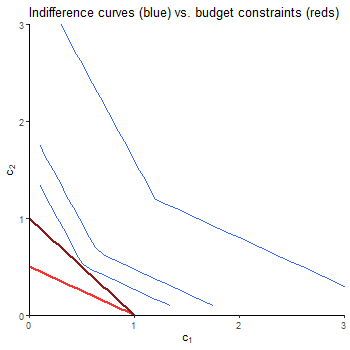
\includegraphics[scale=.6]{2b_IC-and-BC.png}
		\end{center}
		Taken together, the offer curve begins at the boundary solution ($c_2=\frac{p_1}{p_2}w_1$) for all price ratios above a certain level. Around $c_2=2$, the agent becomes indifferent between consuming $c_1$ and $c_2$, with the offer curve following the slope of the indifference curve. However, when $c_1=c_2$, the offer curve hits the kink point of the indifference curve, leading the agent to follow the ridge of the utility function inward, leading to less consumption of both goods as the price ratio decreases (which makes sense, given that the agent only has an endowment of good 1). This continues until the slope of the budget constraint equals to the slope of the indifference cuve, at which point consumption follows the indifference curve until $c_2=0$.
		\begin{center}
			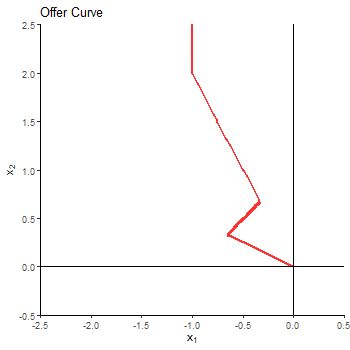
\includegraphics[scale=.6]{2b_offer-curve.png}
		\end{center}
		
	
	\item[(c)] $U=\text{min}\{2c_1+c_2,c_1+2c_2\}$, $(w_1,w_2)=(1,10)$
		\smallskip \\
		This is the same utility function as in 2(b), so the indifference curves have the same shape. The agent has a greater endowment of good 2, so the budget contraints are shifted outward and no longer bounded by 1 on the $c_1$ axis. The offer curve differs from the last example because at the price ratio where $c_1=c_2$ the agent instead follows the ridge of the utility function \textit{outward} as the price ratio increases, which reflects the agent's greater endowment of good 1 than good 2. Since the agent has a nonzero endowment of good one, the offer curve has a boundary solution at $c_2=0$, which continuous as $c_1\rightarrow\infty$.
		\begin{center}
			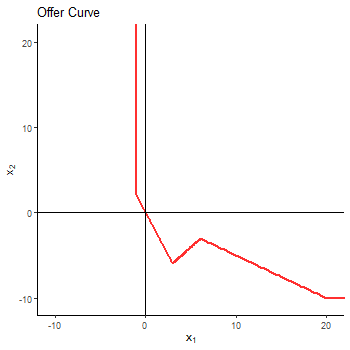
\includegraphics[scale=.6]{2c_offer-curve.png}
		\end{center}
		
	
\end{itemize}



%%%________________________________________________________________%%%


\end{document}












